%\cleardoublepage\newpage\thispagestyle{empty}\null
%\cleardoublepage\newpage\thispagestyle{empty}\null
%\cleardoublepage\newpage
%\thispagestyle{empty}
%\begin{center}
%\Large{To Jung Jae-sung (1982 -- 2018),}
%hello there
%\large{a remarkably hard-working badminton player with a remarkably simple playing style}
%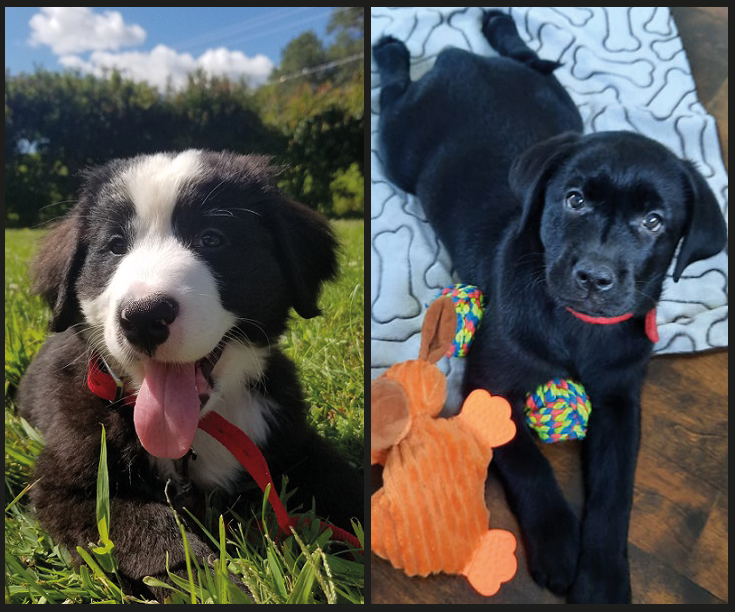
\includegraphics{images/ImageCouverture.png}

%\end{center}

\textbf{Auteurs} : Philippe Apparicio et Jérémy Gelb\\[0.05in]
\textbf{Remerciements} : Ce manuel a été réalisé avec le soutien de la fabriqueREL. Fondée en 2019, la fabrique‑REL est portée par divers établissements d’enseignement supérieur du Québec et agit en collaboration avec les services de soutien pédagogique et les bibliothèques. Son but est de faire des ressources éducatives libres (REL) le matériel privilégié en enseignement supérieur au Québec.\\[0.05in]
\textbf{Maquette de la page couverture} : Graphe Logo (https://www.graphelogo.com/)\\[0.05in]
\textbf{Mise en page} : Philippe Apparicio et Jérémy Gelb\\[0.05in]
\textbf{Relecture} : Denise Latreille\\[0.2in]

© Philippe Apparicio et Jérémy Gelb\\[0.2in]

\textbf{Pour citer cet ouvrage} : Apparicio Philippe et Jérémy Gelb (2022). \textit{Méthodes quantitatives en sciences sociales : un grand bol d’R}. FabriqueREL et Institut national de la recherche scientifique. Licence CC BY‑SA.\\[1in]

\begin{center}
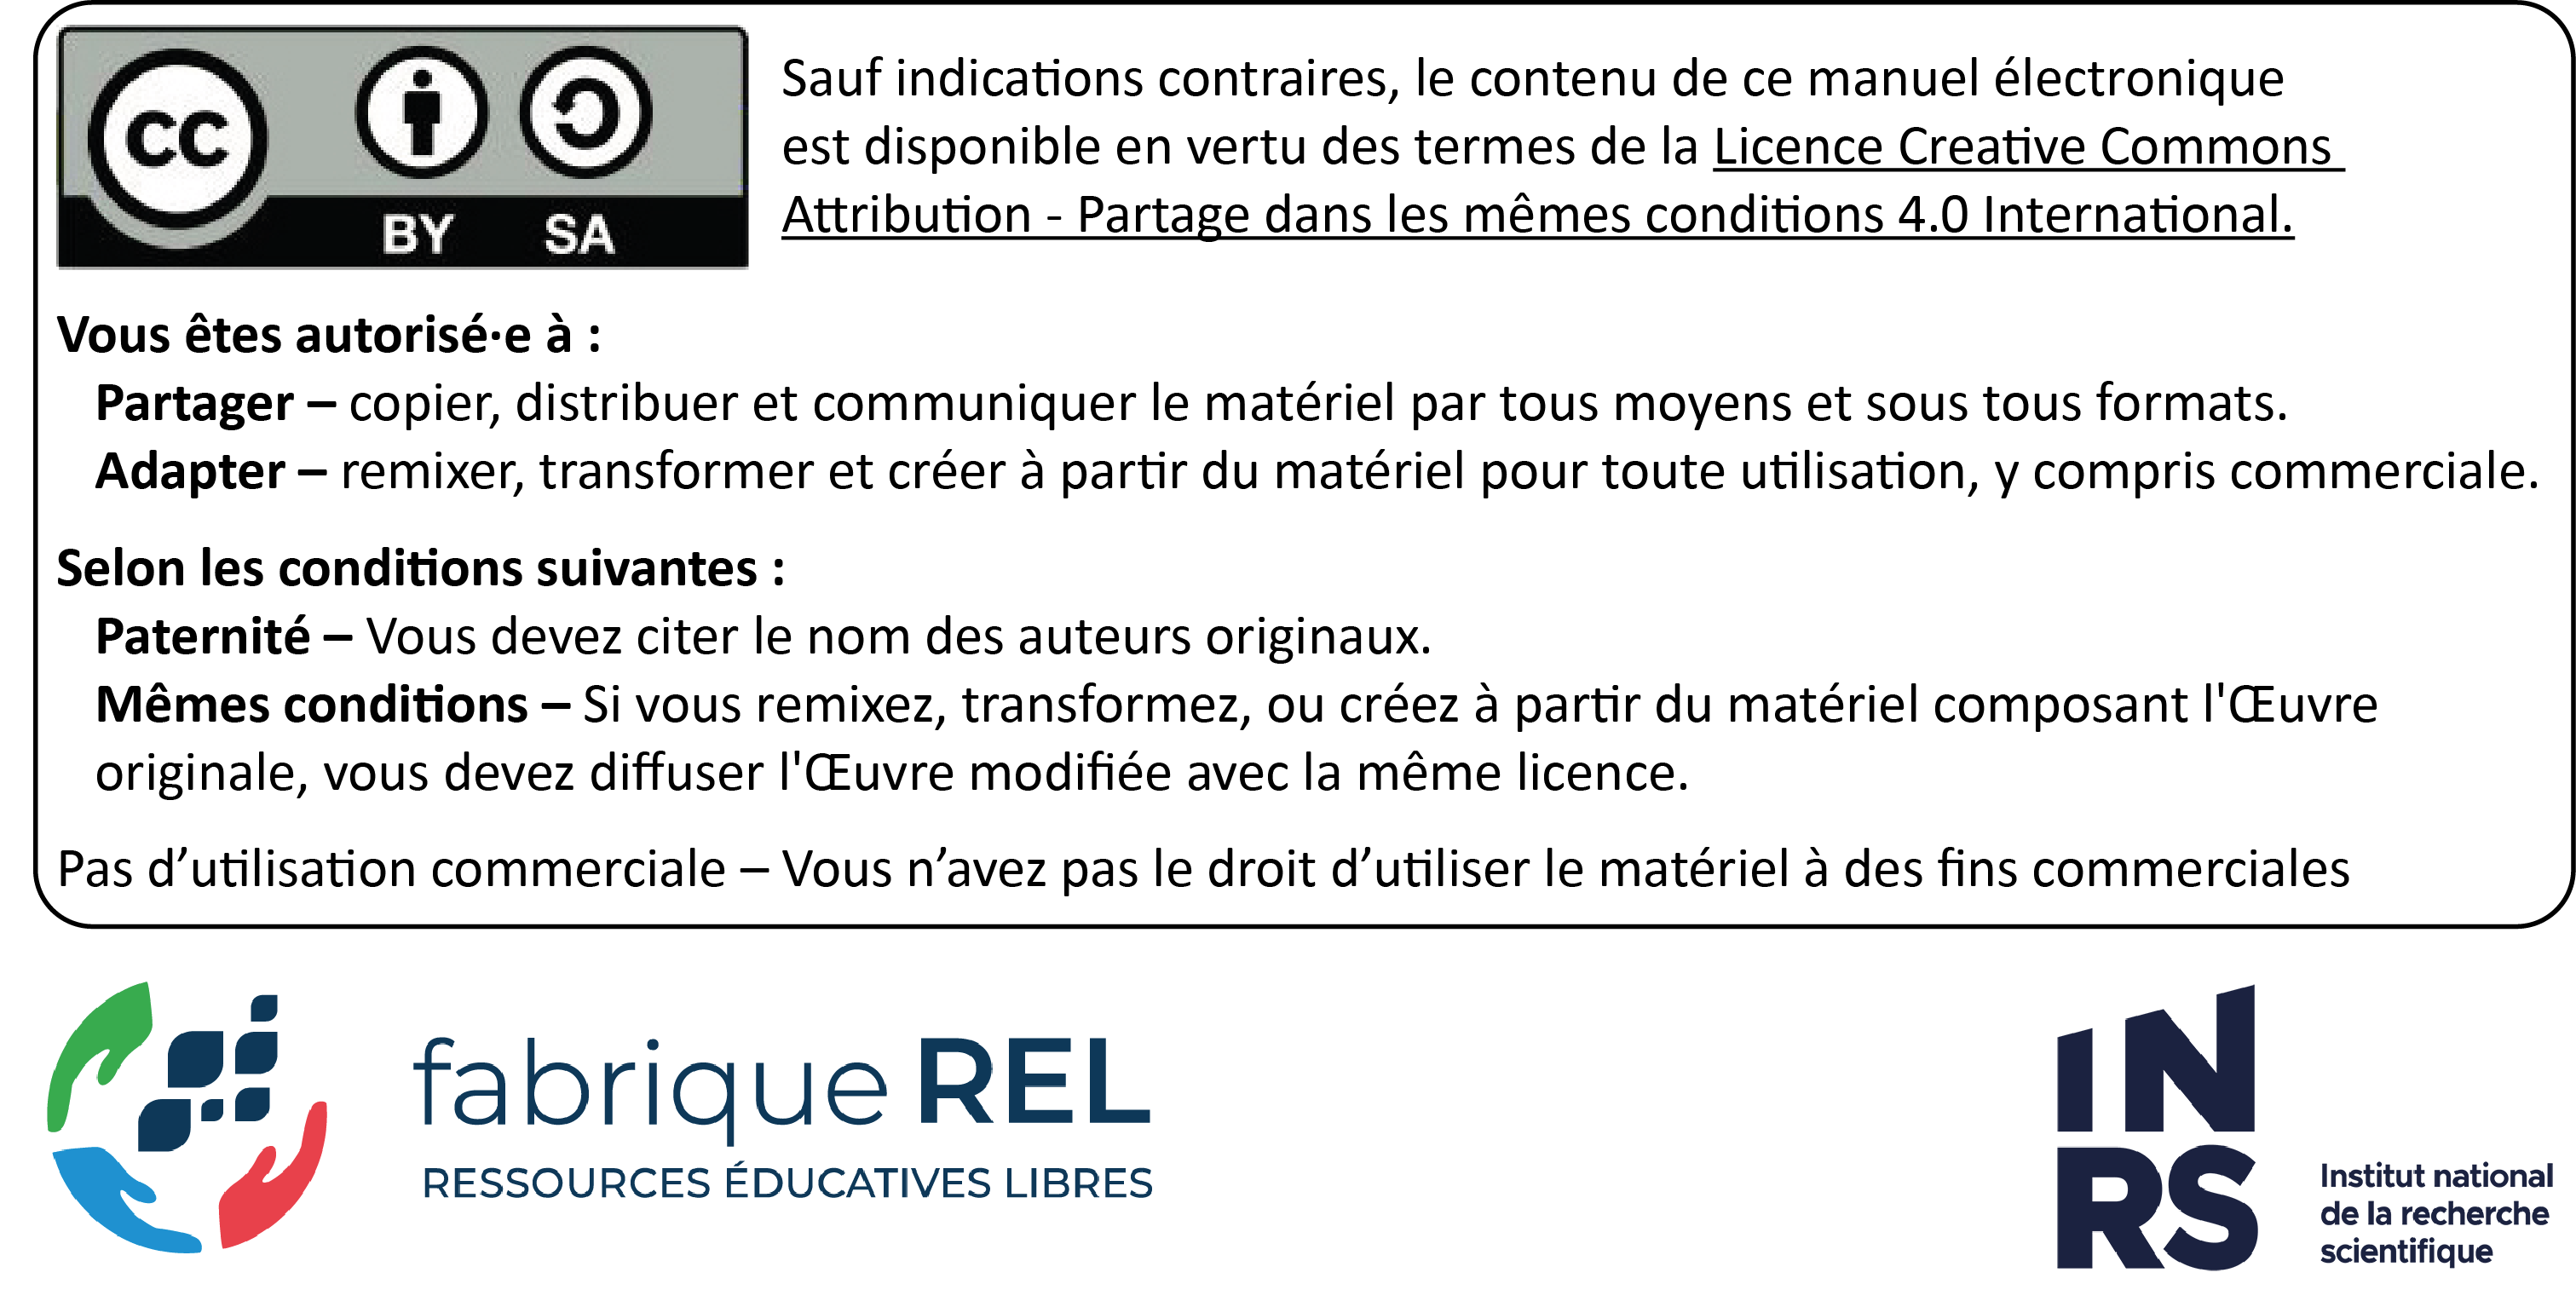
\includegraphics{images/introduction/CouvertureP2.png}
\end{center}

%\let\maketitle\oldmaketitle
%{\let\newpage\relax\maketitle}
%\maketitle



%\setlength{\abovedisplayskip}{-5pt}
%\setlength{\abovedisplayshortskip}{-5pt}
% Setting the name of the lists of figures and tables
\renewcommand*\listfigurename{Liste des figures}
\renewcommand*\listtablename{Liste des tableaux}

%\let\maketitle\oldmaketitle
%\maketitle
